\documentclass[conference]{IEEEtran}
\IEEEoverridecommandlockouts
\usepackage{graphicx}
\usepackage{booktabs}
\usepackage{array}
\usepackage{url}
\usepackage{xcolor}
\usepackage{tikz}
\usetikzlibrary{arrows.meta,positioning,shapes.geometric}
\setlength{\textfloatsep}{7pt plus 2pt minus 2pt}
\setlength{\floatsep}{6pt plus 2pt minus 2pt}
\setlength{\intextsep}{6pt plus 2pt minus 2pt}

\begin{document}
\onecolumn
\pagenumbering{gobble}
\begin{titlepage}
\centering
\vspace*{2cm}
{\Large CSI201 Introduction to Networking\\[0.3cm]
Academic Year 2026/27, Semester 1\par}
\vspace{1.8cm}
{\huge\bfseries NetGuardian: Enterprise SDN Management\par}
\vspace{0.5cm}
{\Large Coursework II\par}
\vspace{1.2cm}
{\Large\color{red}\bfseries DRAFT --- Ubuntu VM measurements and team details pending\par}
\vspace{1.5cm}
\begin{tabular}{ll}
Team / Group: & [Team name or group number] \\
Student 1: & [Full name / pinyin] --- [Student ID] \\
Student 2: & [Full name / pinyin] --- [Student ID] \\
Student 3: & [Full name / pinyin] --- [Student ID] \\
Student 4: & [Full name / pinyin] --- [Student ID] \\
Student 5: & [Full name / pinyin] --- [Student ID] \\
\end{tabular}
\vfill
Submission deadline: 10 December 2026, 23:59\par
\end{titlepage}
\clearpage
\pagenumbering{arabic}
\setcounter{page}{1}
\twocolumn

\title{NetGuardian: Enterprise SDN Management}
\author{\IEEEauthorblockN{[Team name]}
\IEEEauthorblockA{CSI201 Introduction to Networking, AY2026/27 S1}}
\maketitle

\begin{abstract}
This report presents NetGuardian, a Python-based software-defined networking (SDN) management prototype built around Ryu, OpenFlow 1.3, Open vSwitch, and Mininet. The design combines a fixed enterprise topology, MAC-learning forwarding, a guest-to-server access policy, switch-statistics collection, and a threshold detector that temporarily blocks high-rate TCP connection attempts from a designated test host. A VM-oriented experiment runner is provided to check the integrated behavior and collect five performance runs. The implementation and detector unit tests are prepared, but the module Ubuntu VM has not yet been exercised in this draft. Accordingly, measured results, software versions, team details, and evidence references are marked for completion rather than estimated.
\end{abstract}

\begin{IEEEkeywords}
Software-defined networking, OpenFlow, Mininet, network monitoring, intrusion detection
\end{IEEEkeywords}

\section{Introduction}
Traditional networks distribute forwarding decisions among independently configured devices. This can make policy changes and operational monitoring repetitive as an enterprise grows. SDN separates network control logic from packet forwarding and exposes an interface through which a controller can install rules in switches. OpenFlow is one standardized way to communicate those flow rules and statistics to switches [1], [2].

NetGuardian applies this model to a small enterprise network. A Ryu application controls three OpenFlow switches, learns source MAC addresses, and installs forwarding rules. It allows ordinary traffic by default while enforcing one explicit restriction: the guest host h6 cannot reach the protected server h7. A separate security test host, h8, is used to create controlled TCP connections to h7. When the rate of distinct connection tuples passes a configured threshold, the controller adds a temporary higher-priority drop rule. Other clients continue to use the server, and the mitigation rule expires automatically.

The design treats network administration as a sequence of observable control actions. The topology program defines hosts and links; the controller reacts to switch events and packet arrivals; Open vSwitch stores the forwarding state; and the monitoring program samples counters that can be compared with the traffic generator's settings. Keeping these functions in separate modules makes it easier to explain which component owns a failure. For example, a failed ping can be checked against host addressing, MAC learning, the installed policy entry, and controller connectivity rather than diagnosed as one opaque application error.

The coursework has five goals: deploy the specified topology; implement forwarding and access policy; generate traffic and collect flow/port statistics; detect and mitigate abnormal connection creation; and measure four performance metrics over five independent runs. The prototype is intended for functional verification in the supplied Ubuntu VM. Mininet is an emulator, so its results describe this test environment and should not be treated as a prediction of physical-switch performance [3].

The evaluation separates functional checks from quantitative runs. Functional checks establish that the address plan, authorized reachability, guest restriction, monitoring, alert, and timeout recovery behave as intended. Performance runs then repeat the high-rate experiment and record the four metrics specified by the brief. This separation avoids treating a successful single demonstration as evidence of repeatable latency or detection behavior. It also makes the assumptions behind every reported number explicit: the endpoints, observation period, start/end timestamps, and flow-table snapshot must all be stated.

\section{Related Work}
McKeown et al. introduced OpenFlow as a standardized way for a controller to program flow tables in Ethernet switches [1]. The ONF 1.3 specification defines the match fields, priorities, instructions, counters, and timeout behavior used by this implementation [2]. NetGuardian uses those mechanisms directly: a priority-zero table-miss entry sends unmatched packets to Ryu, while higher-priority entries implement policy and forwarding.

Lantz et al. describe Mininet as a rapid SDN prototyping environment that combines host network namespaces, virtual links, and software switches on one machine [3]. This supports repeatable topologies and interactive tests with the same applications and protocol stacks used by the prototype. The single-machine arrangement is also a limitation: timing depends on host scheduling and does not establish production-scale capacity.

Ryu is a component-based framework for building network-control applications and provides an OpenFlow 1.3 API [4]. Its event handlers let NetGuardian respond to switch-feature and packet-in messages, while the packet library exposes Ethernet, IPv4, and TCP headers. The controller uses this event-driven model for MAC learning, five-tuple tracking, and flow installation.

OpenNetMon studies flow-level monitoring in OpenFlow networks and uses switch measurements to derive operational metrics [5]. NetGuardian implements a smaller polling workflow: \texttt{monitoring.py} periodically reads Open vSwitch flow and port counters and records CSV rows and time-series graphs. It does not implement OpenNetMon's measurement algorithms; the work is relevant because it demonstrates why switch counters are useful for network operations.

FRESCO presents a framework for composing OpenFlow-based security detection and mitigation modules [6]. NetGuardian uses the same general control-plane capability in a much narrower form: a single detector counts distinct TCP five-tuples for h8-to-h7 traffic and requests a temporary drop rule. Unlike FRESCO, the coursework prototype has no general module composition, shared security database, or network-wide policy language.

Together, these sources motivate a compact educational design rather than a production security platform. OpenFlow provides the programmable rule interface, Mininet provides a repeatable emulation substrate, and Ryu supplies an event API. Monitoring and security research show how controller visibility can be applied to operational metrics and countermeasures. NetGuardian implements only the narrow subset that the coursework can demonstrate and measure in one VM.

\section{System Design}
\subsection{Topology and components}
The topology has a remote controller c0 at 127.0.0.1:6633 and an s1--s2--s3 switch chain. Hosts h1 and h2 attach to s1; h3, h4, and h5 attach to s2; h6, h7, and h8 attach to s3. h1--h5 represent administrator, staff, and engineering clients. h6 is the guest, h7 is the enterprise server, and h8 is reserved for controlled security experiments. All addresses follow the coursework table.

\begin{figure}[t]
\centering
\resizebox{\columnwidth}{!}{%
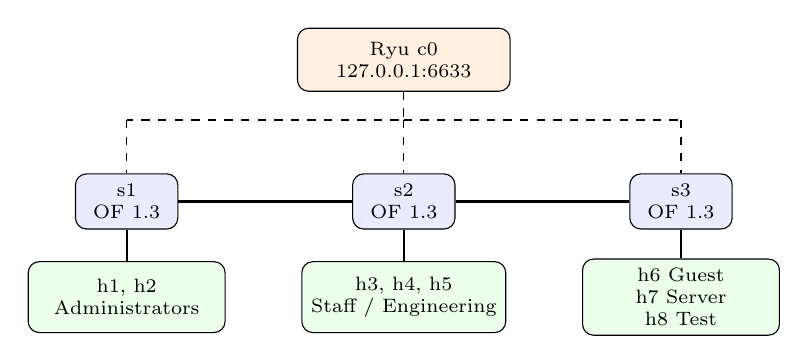
\begin{tikzpicture}[x=11mm,y=9mm,font=\scriptsize,
  sw/.style={draw,rounded corners,minimum width=13mm,minimum height=7mm,fill=blue!8,align=center},
  host/.style={draw,rounded corners,minimum width=25mm,minimum height=9mm,fill=green!8,align=center},
  ctl/.style={draw,rounded corners,minimum width=27mm,minimum height=8mm,fill=orange!12,align=center}]
  \node[ctl] (c) at (3.2,2) {Ryu c0\\127.0.0.1:6633};
  \node[sw] (s1) at (0,0) {s1\\OF 1.3};
  \node[sw] (s2) at (3.2,0) {s2\\OF 1.3};
  \node[sw] (s3) at (6.4,0) {s3\\OF 1.3};
  \coordinate (busl) at (0,1.15); \coordinate (busr) at (6.4,1.15);
  \draw[dashed] (c.south) -- (3.2,1.15) -- (busl);
  \draw[dashed] (3.2,1.15) -- (busr);
  \draw[dashed] (busl) -- (s1.north); \draw[dashed] (3.2,1.15) -- (s2.north);
  \draw[dashed] (busr) -- (s3.north);
  \draw[thick] (s1) -- (s2); \draw[thick] (s2) -- (s3);
  \node[host] (g1) at (0,-1.35) {h1, h2\\Administrators};
  \node[host] (g2) at (3.2,-1.35) {h3, h4, h5\\Staff / Engineering};
  \node[host] (g3) at (6.4,-1.35) {h6 Guest\\h7 Server\\h8 Test};
  \draw[thick] (s1) -- (g1); \draw[thick] (s2) -- (g2); \draw[thick] (s3) -- (g3);
\end{tikzpicture}
}
\caption{NetGuardian topology. Solid lines are data links; dashed lines show controller channels.}
\label{fig:topology}
\end{figure}

\begin{table*}[t]
\caption{Configured host addresses}
\label{tab:hosts}
\centering\small
\begin{tabular}{llll}
\toprule
Host & Role & IPv4 address & MAC address \\
\midrule
h1 & Administrator 1 & 10.0.1.11/16 & 00:00:00:00:01:11 \\
h2 & Administrator 2 & 10.0.1.12/16 & 00:00:00:00:01:12 \\
h3 & Staff 1 & 10.0.2.21/16 & 00:00:00:00:02:11 \\
h4 & Staff 2 & 10.0.2.22/16 & 00:00:00:00:02:12 \\
h5 & Engineering & 10.0.2.23/16 & 00:00:00:00:02:13 \\
h6 & Guest & 10.0.3.31/16 & 00:00:00:00:03:11 \\
h7 & Protected server & 10.0.3.40/16 & 00:00:00:00:03:20 \\
h8 & Security test host & 10.0.3.99/16 & 00:00:00:00:03:99 \\
\bottomrule
\end{tabular}
\end{table*}

\subsection{Forwarding and policy}
\texttt{topology.py} creates the remote controller, switches, fixed-address hosts, and links. In a Task 1 verification, \texttt{learning\_switch.py} provides a policy-free Ryu learning switch so that \texttt{pingall} can test end-to-end connectivity. The main \texttt{controller.py} is used for Tasks 2--5. It keeps a MAC-to-port table for each datapath. On a packet-in, it learns the Ethernet source, looks up the destination, and either floods an unknown destination or installs a rule when the output port is known. TCP forwarding rules match the IPv4 addresses, protocol, and TCP ports so each new connection can reach the controller for flow-rate accounting. Dynamic forwarding entries use a five-second idle timeout; the table-miss entry is permanent.

The default policy permits IPv4 communication except h6-to-h7. A priority-400 drop entry on s3 matches the guest and server IP addresses and is installed when s3 connects. The reverse direction and other source/destination pairs remain eligible for ordinary learning-switch forwarding. This ordering ensures that the first guest packet cannot pass before the policy is installed.

\begin{table}[t]
\caption{NetGuardian communication policy}
\label{tab:policy}
\centering\small
\begin{tabular}{lll}
\toprule
Source & Destination & Action \\
\midrule
h1--h5 & h7 & Allow \\
h6 & h7 & Drop (priority 400) \\
h6 & Other hosts & Allow \\
h8 & h7, normal rate & Allow \\
h8 & h7, over threshold & Temporary drop (priority 500) \\
\bottomrule
\end{tabular}
\end{table}

\subsection{Packet processing and rule lifecycle}
When a switch connects, Ryu receives a switch-features event and installs the table-miss entry. That entry outputs unmatched packets to the controller and has no idle timeout. At s3, the controller also installs the fixed guest policy drop. For ordinary Ethernet traffic, a packet-in causes the application to record the source MAC and ingress port in the map belonging to that datapath. If the destination has not been learned on that switch, the packet is flooded so that the destination can respond. When the destination becomes known, the controller sends a packet-out for the current packet and adds a matching forwarding entry for subsequent traffic.

The topology is a tree, so flooding across the inter-switch links has no cyclic path. ARP is flooded to let hosts resolve the fixed IPv4 addresses before the controller can learn unicast endpoints. The table-miss entry remains as the fallback when temporary entries expire. The ordinary dynamic rules use an idle timeout of five seconds, which bounds stale forwarding state. Security rules have separate lifetime semantics: the guest policy is persistent, while the intrusion-mitigation rule uses a finite hard timeout as required by Task 4.

For TCP, the forwarding match includes source IP, destination IP, IP protocol, source TCP port, and destination TCP port. A rule that matched only the two IP addresses would hide later connections from the controller until that rule expired. Matching the ports retains per-connection visibility: packets in an existing tuple use the switch entry, but a new source port produces a packet-in and can be counted. The detector state is scoped to h8-to-h7 TCP; normal clients and other destinations do not contribute to the suspicious-flow threshold.

\subsection{Monitoring and security response}
\texttt{monitoring.py} polls \texttt{ovs-ofctl} once per interval for each switch. It records a timestamp, switch identifier, packet/byte counters, maximum active-flow duration, active non-table-miss flow count, and aggregate receive/transmit port-packet counters. It writes CSV files and plots active flows and cumulative flow bytes over successive samples. Flow byte counters are cumulative, so a change between samples indicates traffic volume during that interval.

The controller observes h8-to-h7 TCP packet-in events and identifies each connection by (source IP, destination IP, source port, destination port, protocol). A candidate packet-in is counted after a subsequent s3 OpenFlow flow-stat reply confirms the corresponding five-tuple forwarding entry. A five-second rolling set counts each distinct confirmed tuple once while it remains in the window. The rate is count divided by five seconds. With the default threshold of four new flows/s, a count of 20 is at the threshold and 21 exceeds it. This is a configurable demonstration threshold, not a universal attack boundary. Each confirmed observation is appended to \texttt{security\_events.csv}, with the current active h8-to-h7 flow count from the same statistics snapshot; an over-threshold observation logs an alert and installs a priority-500 drop rule for h8-to-h7 with a 15-second hard timeout. The rule outranks forwarding and the guest policy. After expiry, h8 can be tested again without manual rule removal.

The controller logs the UTC timestamp, source host and IP, destination IP, ports, protocol, window length, distinct-flow count, measured rate, threshold, active matching-flow count, alert flag, and action. The threshold comparison is strict: a measured rate equal to the threshold does not trigger. Once mitigation begins, the aggregate source/destination rule matches all IPv4 traffic from h8 to h7, not just TCP port 5001, which also makes the blocked state easy to verify with ICMP. The rule's higher priority ensures it takes precedence over ordinary forwarding. Legitimate hosts remain outside its match, so their server traffic should continue during the test.

\begin{figure}[t]
\centering
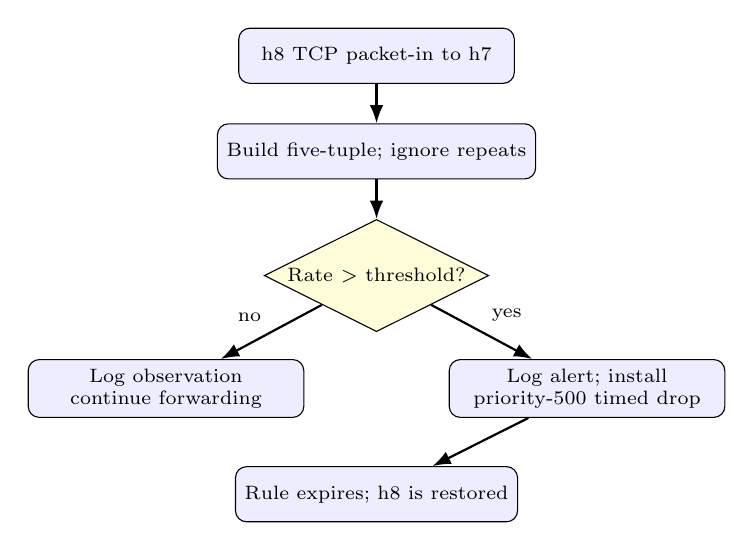
\begin{tikzpicture}[font=\scriptsize,node distance=5mm,
  box/.style={draw,rounded corners,align=center,minimum width=35mm,minimum height=7mm,fill=blue!7},
  decision/.style={draw,diamond,aspect=2,align=center,inner sep=1pt,fill=yellow!15},
  arr/.style={-{Latex},thick}]
  \node[box] (pkt) {h8 TCP packet-in to h7};
  \node[box,below=of pkt] (tuple) {Build five-tuple; ignore repeats};
  \node[decision,below=of tuple] (rate) {Rate $>$ threshold?};
  \node[box,below left=7mm and 2mm of rate] (normal) {Log observation\\continue forwarding};
  \node[box,below right=7mm and 2mm of rate] (drop) {Log alert; install\\priority-500 timed drop};
  \node[box,below=17mm of rate] (expire) {Rule expires; h8 is restored};
  \draw[arr] (pkt)--(tuple); \draw[arr] (tuple)--(rate);
  \draw[arr] (rate)--node[above left]{no}(normal);
  \draw[arr] (rate)--node[above right]{yes}(drop);
  \draw[arr] (drop)--(expire);
\end{tikzpicture}
\caption{New-flow detection and timeout-based recovery.}
\label{fig:ids}
\end{figure}

\section{Implementation}
The target environment is the module-provided Ubuntu VM with Python 3, Mininet, Ryu, and Open vSwitch. Exact installed versions and VM kernel details are to be recorded from the validated run and inserted here: [Ubuntu/kernel: pending]; [Python: pending]; [Mininet: pending]; [Ryu: pending]; [Open vSwitch: pending]. The topology configures OpenFlow 1.3 and uses the controller address and port shown in the coursework figure.

The code is divided by responsibility. \texttt{topology.py} builds and starts the Mininet network. \texttt{learning\_switch.py} is a Task 1-only controller without the guest restriction. \texttt{controller.py} handles switch events, per-switch MAC learning, policy enforcement, five-tuple detection, CSV alert logging, and timed mitigation. \texttt{flow\_detection.py} is a small standard-library rolling-window component that can be tested without Ryu. \texttt{traffic\_generator.py} produces ICMP echo attempts or TCP connection attempts at a chosen rate and duration. TCP tests use a Python HTTP service on h7. \texttt{monitoring.py} polls flow and port counters and produces CSV and labeled SVG graphs without requiring an extra package; it also produces PNG graphs if Matplotlib is already available. \texttt{experiment.py --live} starts the controller, topology, traffic, monitoring, and five-run evaluation in the VM, then writes results and a transcript to unique output paths.

The detection window and threshold were selected to distinguish the demonstrated rates: one new connection per second remains below the threshold, whereas an eight-per-second generator should exceed it within a five-second window. A 15-second hard timeout is long enough to verify the block while permitting automatic recovery during a short demonstration. These settings require validation against the actual VM; the threshold may need adjustment if connection attempts are delayed or coalesced by the environment. The implementation handles the Task 4 mitigation and guest rule at s3 because h6, h7, and h8 attach to that switch.

The traffic generator accepts a mode, destination address, rate, duration, and TCP port. ICMP mode invokes one-packet ping attempts at the requested cadence; TCP mode repeatedly opens and closes client connections. The high-rate experiment is therefore a connection-creation workload, not a sustained bulk-data transfer. That distinction matters when interpreting counters: short connections increase the number of flow entries and packet-in events, while the total byte count can remain modest. The web server on h7 provides a listening endpoint for connection establishment and can be started without installing a separate service package.

\texttt{monitoring.py} runs outside the Mininet host namespaces and queries each named OVS bridge. Flow output provides packet and byte counters, durations, and match entries; port output provides receive and transmit packet counts. Active flows exclude the priority-zero table-miss entry. The monitoring CSV has one flow row and one port row per switch and sample time. The active-flow graph plots the count for each switch, while the traffic-volume graph plots cumulative bytes. Both graphs use sample number on the horizontal axis so that irregular VM scheduling does not imply a more precise clock than the data supports. The SVG writer uses only the standard library; PNG output is supplemental when Matplotlib is preinstalled in the module VM.

The integrated runner records unique output files so that successive experiments do not silently replace earlier results. Its transcript records host addresses, bridge protocols, initial flows, policy checks, each performance run, and output locations. The Ryu log is retained separately to make the alert timestamp and switch connection messages auditable. For a formal report, the evidence set should keep the CSVs and graphs alongside readable terminal screenshots rather than relying on the runner's summary alone.

One design issue is the relationship between flow visibility and forwarding. A broad TCP flow rule would allow later connections to bypass packet-in and make new-connection counting incomplete. The controller therefore matches TCP source and destination ports as well as IP addresses and protocol. This yields a packet-in for a new five-tuple while letting later packets in the same connection use the installed rule. The trade-off is more short-lived flow entries, controlled here by the five-second idle timeout.

\section{Testing and Results}
The standard-library unit tests check tuple deduplication, strict threshold comparison, rolling-window expiry, detector validation, labeled SVG generation, ping metric parsing, and CSV handling. On the development host, nine tests passed under Python 3.13.2. This is not a substitute for the required module Ubuntu VM validation. The actual VM run, flow tables, screenshots, generated CSVs, graphs, and five measurements remain pending in this draft.

The live VM workflow first checks authorized reachability (h1 to h7), guest denial (h6 to h7), and guest access to a non-protected client (h6 to h1). It then starts the HTTP server and monitoring poller, runs ICMP and ordinary TCP traffic, checks that low-rate h8 traffic is not flagged, and conducts five high-rate trials. For each performance run, it records mean RTT from h1-to-h7 ping output before abnormal traffic, the aggregate active non-table-miss flow count around detection, time from abnormal traffic start to the alert timestamp, and time from alert observation to visibility of the drop rule in the s3 flow table. During each mitigation it checks that h1 can still reach h7, that h8 cannot, and that h8 recovers after rule expiry.

Each run should be treated as independent only after the prior mitigation has expired and the detector's five-second state window has drained. The runner waits for the finite rule to disappear, verifies h8 recovery, and leaves a quiet interval before starting the next trial. RTT is measured before the abnormal workload so that it represents normal operation. Active-flow count is a point-in-time sum across s1--s3 near the alert and therefore depends on the sampling instant; the method should be kept consistent across all five runs. Detection time uses the controller's logged alert timestamp, and mitigation response is measured by polling the s3 table until the priority-500 entry appears. The polling interval imposes a small observation bound on that response metric, which should be acknowledged when discussing very short delays.

\subsection{Evidence scope and validity}
Task 1 and the integrated test use different controller configurations for a reason. The policy-free learning switch is used for the required all-hosts \texttt{pingall} check. In the integrated NetGuardian run, h6-to-h7 loss is the expected result of the guest policy, so \texttt{pingall} is not a success criterion for that configuration. The specific policy tests are more informative: an authorized client reaches h7, h6 is denied by the guest rule, and h6 can still reach a non-protected host. Flow tables should be captured both immediately after traffic and after a six-second quiet period to show that ordinary five-second idle entries expire while table-miss and policy entries remain.

The abnormal workload consists of connection attempts, not payload-intensive data transfer. Its rate controls how often the client opens a TCP socket; it does not emulate every property of a real attack. Packet-in timing and the flow-stat polling period affect how quickly the controller confirms a new entry, while VM CPU contention can add variation. The reported detection time therefore describes this specific traffic generator and VM. The threshold should be discussed as a chosen experimental decision boundary, including the demonstrated low and high rates, rather than as a general classifier for malicious traffic.

The evidence should corroborate each stage with the relevant source. Mininet's \texttt{nodes}, \texttt{net}, and \texttt{dump} outputs establish deployment; \texttt{pingall} establishes Task 1 reachability; \texttt{ovs-vsctl} confirms OpenFlow 1.3; and \texttt{ovs-ofctl dump-flows} shows the actual rules and timeouts. Controller logs show MAC learning and alerts. Monitoring CSVs and graphs show switch counters over time. The performance CSV preserves each trial's metrics, while screenshots and the video make the order of operations visible. These artifacts should use matching run timestamps where possible so that the alert, flow table, and measurement rows can be associated with the same experiment.

The report should include the controller and OVS versions, the exact threshold/window/timeout, five individual values, their arithmetic means, and a brief discussion of run-to-run spread. If one trial fails a functional assertion, it should be rerun after diagnosing the cause, and the retained table should contain five valid independent runs. Screenshots should show readable terminal output and timestamps. No values should be inferred from the default configuration or from the unit tests.

\begin{table}[t]
\caption{Five independent performance runs (replace after VM execution)}
\label{tab:results}
\centering\scriptsize
\begin{tabular}{rrrrr}
\toprule
Run & RTT (ms) & Flows & Detect (s) & Mitigate (s) \\
\midrule
1 & [pending] & [pending] & [pending] & [pending] \\
2 & [pending] & [pending] & [pending] & [pending] \\
3 & [pending] & [pending] & [pending] & [pending] \\
4 & [pending] & [pending] & [pending] & [pending] \\
5 & [pending] & [pending] & [pending] & [pending] \\
Mean & [pending] & [pending] & [pending] & [pending] \\
\bottomrule
\end{tabular}
\end{table}

Observed traffic differences, detection effectiveness, legitimate-host availability during mitigation, restoration, and variation between runs must be summarized from the real VM evidence here: [findings pending]. Attach or cite evidence for the Task 1 topology and full \texttt{pingall}; Task 2 forwarding and policy flows; Task 3 traffic, counters, CSVs, and graphs; Task 4 low/high-rate event records and recovery; and Task 5 integrated behavior and five-run table. Do not retain this paragraph or the pending table in the submitted report.

\subsection{Results interpretation and validity}
The final discussion should compare the normal client experiments with the h8 workload using the same measurement interval. A rise in distinct active flows is direct evidence that connection attempts reached the forwarding plane; a change in cumulative byte counters shows how much traffic those flows carried. Since the generator opens short-lived TCP sockets, the high-rate case is expected to create more flow entries than a low-rate case even when its byte volume is not proportionally large. The actual CSV and graph values must determine whether that pattern occurred in the VM run.

Detection effectiveness should be reported as an observed outcome for both controlled rates. For the low-rate trial, give the maximum measured rate and state whether any alert row appeared. For the high-rate trial, quote the alert's measured rate, threshold, and time to detection. If the controller missed a threshold crossing, examine whether the switch statistics replies confirmed the five-tuple rules, whether the TCP service was listening, and whether the traffic generator achieved its configured cadence. These checks separate an IDS issue from a failed traffic setup.

Mitigation is successful only if the priority-500 rule is visible and packet behavior matches it. Report the h8-to-h7 result while the rule is active, the h1-to-h7 result during the same period, and h8's result after expiry. A drop entry alone does not prove legitimate service availability, and a failed ping after expiry may indicate stale ARP, a server issue, or a separate forwarding problem. The integrated runner checks these conditions explicitly, but the screenshots and flow table should be retained as corroborating evidence.

For the five-run analysis, list all measurements before discussing the mean. Compare the spread rather than presenting the average as a guarantee. RTT may vary with VM scheduling; active-flow count varies with the exact snapshot time and entries expiring; detection time includes the statistics polling cadence; and mitigation response is bounded by the rule-table polling interval. Report the configured cadence and acknowledge this measurement resolution. If one run differs sharply, inspect the corresponding event and flow-table logs instead of removing it without explanation. All numerical claims should be traceable to one of the saved run files.

\section{Conclusion}
NetGuardian combines programmable topology deployment, OpenFlow learning and policy rules, polling-based monitoring, and threshold-triggered temporary mitigation. The prepared implementation emphasizes short-lived per-connection forwarding entries so the controller can observe new TCP tuples, while a higher-priority timed rule blocks the designated test host without stopping legitimate clients. The conclusions about execution correctness and measured latency must be completed after validating the integrated workflow on the course VM. Further work could add adaptive thresholds, richer event aggregation, controller-side statistics polling, and tests on larger or physical networks.

\section*{Acknowledgment}
[Full name] ([Student ID]): [contribution]%; repeat for every team member. Percentages must total 100\%.

\clearpage
\begin{thebibliography}{00}
\bibitem{openflow-intro} N. McKeown, T. Anderson, H. Balakrishnan, G. Parulkar, L. Peterson, J. Rexford, S. Shenker, and J. Turner, ``OpenFlow: Enabling Innovation in Campus Networks,'' \emph{ACM SIGCOMM Computer Communication Review}, vol. 38, no. 2, pp. 69--74, Apr. 2008.
\bibitem{openflow-spec} Open Networking Foundation, \emph{OpenFlow Switch Specification, Version 1.3.0}, ONF TS-006, June 2012. [Online]. Available: \url{https://opennetworking.org/wp-content/uploads/2014/10/openflow-spec-v1.3.0.pdf}
\bibitem{mininet} B. Lantz, B. Heller, and N. McKeown, ``A Network in a Laptop: Rapid Prototyping for Software-Defined Networks,'' in \emph{Proc. 9th ACM SIGCOMM Workshop on Hot Topics in Networks (HotNets-IX)}, Monterey, CA, USA, 2010.
\bibitem{ryu} Ryu Project, ``Ryu SDN Framework: OpenFlow 1.3 API Reference.'' [Online]. Available: \url{https://ryu.readthedocs.io/en/latest/ofproto_v1_3_ref.html}
\bibitem{opennetmon} N. L. M. van Adrichem, C. Doerr, and F. A. Kuipers, ``OpenNetMon: Network Monitoring in OpenFlow Software-Defined Networks,'' in \emph{Proc. IEEE/IFIP Network Operations and Management Symposium (NOMS)}, Krakow, Poland, 2014, pp. 1--8, doi: 10.1109/NOMS.2014.6838228.
\bibitem{fresco} S. Shin, P. Porras, V. Yegneswaran, M. Fong, G. Gu, and M. Tyson, ``FRESCO: Modular Composable Security Services for Software-Defined Networks,'' in \emph{Proc. Network and Distributed System Security Symposium (NDSS)}, San Diego, CA, USA, 2013.
\end{thebibliography}
\end{document}
